\section{Clasificadores}

En la presente sección se describen brevemente algunos clasificadores utilizados en la tesina para encontrar un primer punto de partida (\textit{baseline}) contra el cuál comparar el desarrollo posterior.

\textit{\textbf{Support Vector Machine}} (SVM) es utilizado en \cite{tesis-parodi}, sobre el cuál nuestro trabajo se ha basado fuertemente. También hemos experimentado utilizando \textit{\textbf{Random Forest}} (RF) sobre las características extraídas en el mencionado trabajo.

\textbf{Redes Neuronales Artificiales} (a pesar de ser un clasificador) será desarrollado en la sección siguiente ya que es el método principal utilizado por nuestro trabajo.

\subsection{Random Forest}

\subsubsection{Árboles de Decisión}

Los árboles de decisión son un método simple que consiste en particionar recursivamente mediante hiperplanos el espacio de atributos de modo que quede finalmente partido en hiper-rectángulos \cite{Hastie}. A cada región se le asigna un valor de predicción constante. A la hora de realizar una inferencia sobre un ejemplo $x$ primero se ubicará la región a la que pertenece. Esto puede hacerse siguiendo las reglas de particionado del árbol de decisión binaria que generó las regiones. Finalmente, la predicción será la predicción constante de dicha región. En general el valor constante óptimo para cada región (ajustado sobre el conjunto de datos de entrenamiento) es tomar la media de la variable dependiente $\bar{y}$ en problemas de regresión que usan $MSE$ como métrica, o tomar la etiqueta más frecuente (moda) de las $y_i$ en problemas de clasificación que usan $Error~Rate$ como métrica. Ver figura \ref{fig:randomforest}.

\begin{figure}[h!] 

\centering
\begin{subfigure}{0.33\textwidth}
\centering 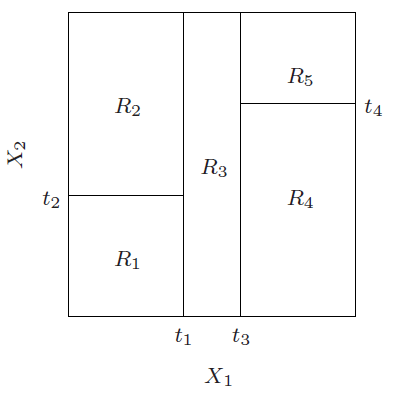
\includegraphics[width=0.3\textwidth]{imgs/decision_tree_1.png}
\end{subfigure}
\begin{subfigure}{0.33\textwidth}
\centering 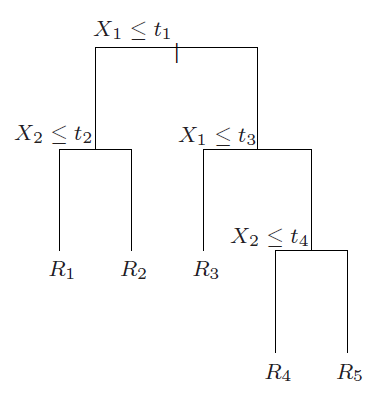
\includegraphics[width=0.3\textwidth]{imgs/decision_tree_2.png}
\end{subfigure}
\begin{subfigure}{0.33\textwidth}
\centering 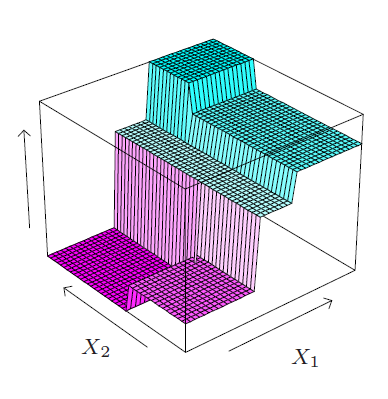
\includegraphics[width=0.3\textwidth]{imgs/decision_tree_3.png}
\end{subfigure}

\caption{ A la izquierda se muestra el espacio de atributos partido en regiones. En el centro se muestra el particionado recursivo (arbol de decisión binaria) que dio como resultado dichas regiones. A la derecha se muestra la función de predicción del modelo que asigna para cada región valores constantes. }
\label{fig:randomforest}
\end{figure}

\subsubsection{\textit{Classification And Regression Tree (CART)}}

El algoritmo de CART es uno de los métodos más populares para construir árboles de decisión. Otras opciones son los métodos ID3 \cite{rf-id3}, C4.5 \cite{rf-c4} y C5.0 \cite{rf-c5}.\\

Para explicar el algoritmo supongamos que tenemos $N$ ejemplos de entrenamiento:
\begin{equation*}
    \{(x_i, y_i), 1 \leq i \leq N\}
\end{equation*}
A su vez consideremos que la variable independiente posee $p$ atributos:
\begin{equation*}
    x_i = ( x_{i,1}, x_{i,2}, ... x_{i,p} ), 1 \leq i \leq N
\end{equation*}

Una partición sobre el atributo $j$ y valor de división $s$ define las regiones $R_1$ y $R_2$ según:
\begin{equation*}
    R_1(j,s) = \{ x | x_{i,j} \leq s, 1 \leq i \leq N \}
\end{equation*}
\begin{equation*}
    R_2(j,s) = \{ x | x_{i,j} > s, 1 \leq i \leq N \}
\end{equation*}
A su vez las predicciones para dichas regiones serán $c_1$ y $c_2$ calculadas como ya se explicó.\\

Para encontrar la mejor partición binaria se optimiza:

\begin{equation*}
    min_{j,s} [ \sum_{x_i \in R_1(j,s)} criterion(y_i, c_1) + \sum_{x_i \in R_2(j,s)} criterion(y_i, c_2) ]
\end{equation*}
Los criterios más usados son $MSE$ para problemas de regresión o \textit{Gini Impurity} o \textit{Information Gain} \cite{rf-inf-gain} para problemas de clasificación.

Para cada uno de los $p$ atributos se puede ordenar en los ejemplos según su $j$-ésima feature con una complejidad de $\mathcal{O}(N~log~N)$  y luego encontrar el mejor valor de división $s$ con una complejidad $\mathcal{O}(N)$. Haciendo esto para cada atributo $j$ se puede encontrar la mejor elección de $s$ sumando una complejidad total de: $\mathcal{O}(p N~log~N)$) en cada paso de subdivisión nueva del árbol. Incluso se puede ordenar una vez al principio y mantener $p$ listas (una para cada atributo) de índices que apunten a los $x_i$ ordenada según dicho $j$-ésimo atributo, ahorrando el factor $log N$ en cada paso.

El algoritmo CART encuentra la mejor partición binaria, se particionan los datos en las regiones resultantes y se repite recursivamente el proceso de división. La decisión de partir en la mejor partición en cada paso es una decisión \textit{greedy}. Optimiza la mejor decisión local, o sea en un único paso de subdivisión, aunque puede no ser la mejor decisión global, o dicho de manera más coloquial ``al largo plazo''. De todas formas llega a muy buenos resultados de árboles de decisión. \\

\textbf{Ventajas de los Árboles de Decisión:} 
\begin{itemize}
    \item Poseen bajo sesgo, pués no hacen demasiadas asumpciones en la función objetivo.
    \item Son simples, no poseen demasiados hiperparámetros a ajustar.
    \item Son robustos al escalado de los atributos. No requieren normalizar o estandarizar los datos. Son insensibles a estos preprocesamientos puesto que sólo importa el orden de los características, no su escala.
\end{itemize}

\textbf{Desventajas de los Árboles de Decisión:}
\begin{itemize}
    \item Los árboles profundos poseen alta varianza, por lo cuál, de no configurar bien los hiperparámetros que controlan su complejidad (cantidad mínima de nodos, profundidad máxima o aplicar técncias de podas) son propensos a sobreajustar.
    \item Al predecir valores constante para cada región son incapaces de descubrir tendencias que permitan extrapolar las predicciones a rangos de atributos que no estén dentro del rango de los atributos presente en el conjunto de entrenamiento; potencialmente arrojando resultados erróneos para ellos. Ver figura \ref{fig:rf-extrapolation-problem}.
    
    A diferencia de lo que muchos creen, no es un problema que tengan sólo en problemas de regresión sino que se pueden pensar casos en donde afecten a problemas de clasificación (por ejemplo distinguir la clase de los $(x_1,x_2)$ donde $|x_1 - x_2 | \leq 1$). Y es que la escencia del problema radica en que las regiones con valores constantes no predicen bien ejemplos que poseean atributos ``más allá'' de los rangos de los atributos presentes en el entrenamiento.
\end{itemize}

\subsubsection{\textit{Random Forest}}

Para mitigar el problema de la alta varianza de los árboles de decisión se puede recurrir a \textit{\textbf{decision tree bagging}}. En este método se entrena un número $t$ de árboles de decisión, cada uno basado en diferentes subconjuntos de $m$ ejemplos tomados del conjunto de datos de entrenamiento y luego (para la inferencia) se combinanan los resultados de las predicciones, por ejemplo, tomando la media o moda. Cuándo se combinan modelos se suele hablar de \textit{\textbf{ensamble}}.

Esta técnica es denominada \textit{\textbf{Bagging}} y puede aplicarse sobre cualquier predictor \cite{breiman-1993}. Es un caso particular de la técnica denominada \textit{\textbf{Bootstrap}}, utilizada para encontrar buenos estimadores estadísticos sobre una población \cite{Hastie}. Tiene la capacidad de reducir dramáticamente la varianza de predictores inestables como árboles de decisión sin introducir sesgo, lo cual conduce a mejores resultados. Una propiedad importante de los \textit{ensambles} es que al incrementar el número $t$ de estimadores base utilizados, el valor de la predicción no puede empeorar. Como  contrapartida, la construcción será más lenta (un factor lineal respecto de $t$). \\

\textit{\textbf{Random Forest}} es una modificación de un \textit{\textbf{decision tree bagging}} donde además de la técnica de \textit{bagging} se agrega que, cuando se crean los árboles de decisión, en cada nivel a subdividir se consideran aleatoriamente sólo $k$ de los $p$ atributos como candidatos. Ésto introduce ruido en el proceso que ayuda a que los $t$ árboles generados no estén tan correlacionados, reduciendo aún más la varianza del \textit{ensamble}. \cite{breiman-2001}. 
Valores pequeños de $k$ reducirán la correlación entre cada par de árboles del ensamble, y por lo tanto, reducirán la varianza en promedio. Generalmente se toma $k = \sqrt{p}$. \\

\textbf{OOB (\textit{out of bag}):} para cada ejemplo $x_i$ del conjunto de datos, es posible construir una predición de \textit{Random Forest} promediando sólo las predicciones de aquellos árboles que no incluyeron a $x_i$ en el conjunto de entrenamiento. Esto es lo que se conoce como \textit{\textbf{OOB score}}. El \textit{OOB score} constituye una métricas de validación correcta y es calculada haciendo uso de elementos incluídos en el conjunto de entrenamiento, lo que implica que no necesitamos reservar datos para la validación. ¡Podemos entranar con todos los datos!.

Es importante notar que si el \textit{Random Forest} posee $t$ predictores, durante el cálculo del \textit{OOB score} se utiliza para cada ejemplo una cantidad menor de predictores (ya que se obvian para cada ejemplo los que lo utilizaron para entrenar). Es por ello que el \textit{OOB score} será una métrica \textit{pesimista} (se pueden esperar mejores resultados sobre un conjunto de test). También es importante aclarar que al igual que el método de \textit{Cross-Validation}, \textit{OOB Score} se basa en la asumpción de que un particionado aleatorio del conjunto de datos constituye una buen conjunto de validación. De no ser cierto esto observaremos un considerablemente mejor \textit{OOB score} que los resultados observados sobre un conjunto de test bien confeccionado.\\

\textbf{Ventajas de \textit{Random Forest}:} tienen la simplicidad de los árboles de decisión (pocos hiperparámetros, insensible a la escala de atributos) y respecto a los mismos, resuelve el problema de sobreajuste causado por la alta varianza.\\

\textbf{Desventaja de \textit{Random Forest}:} no solucionan el problema de extrapolación que poseen los árboles de decisión. Ver figura \ref{fig:rf-extrapolation-problem}.

\begin{figure}[h]
\centering
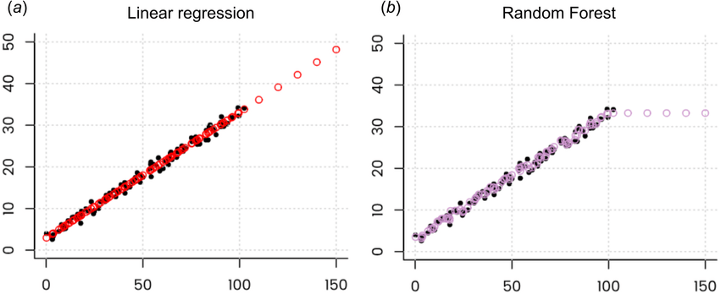
\includegraphics[width=0.9\textwidth]{imgs/rf_extrapolation_problem.png}
\caption{Ejemplo del problema de extrapolación que poseen los árboles de decisión y hereda el método de Random Forest. Créditos: Derrick Mwiti \url{https://neptune.ai/blog/random-forest-regression-when-does-it-fail-and-why} }
\label{fig:rf-extrapolation-problem}
\end{figure}






\subsection{Support Vector Machine}

Las Máquinas de Vectores Soporte son un método de clasificación que está sustentada por un desarrollo matemático teórico de envergadura ya que se basa en aprendizaje estadístico o teoría VC (Vapnik-Chervonenkis) \cite{svm-vapnik1}, \cite{svm-vapnik2}.\\

Procederemos a explicar intuitivamente y de manera sencilla las ideas claves. Atiunque haremos referencias a las formulaciones matemáticas, no profundizaremos en ellas. El lector puede ampliar sobre el desarrollo del método leyendo \cite{svm-genesis1} \cite{svm-genesis2} o ahondar en el desarrollo matemático en \cite{Hastie}.

\begin{enumerate}
    \item Una tarea de clasificacióin puede ser vista como la tarea de separar los espacios geométricos que ocupa cada clase dentro del espacio de atributos. Ver figura \ref{fig:svm-seperadores}.
    
\begin{figure}[h!]
\centering
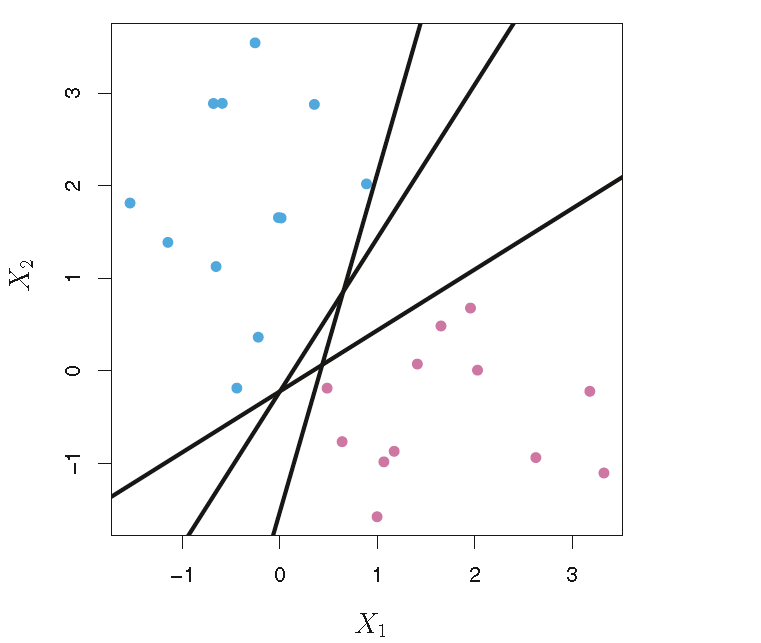
\includegraphics[width=0.45\textwidth]{imgs/svm_separadores.png}
\caption{ Ejemplo de clasificación binaria particionando el espacio geométrico de atributos por medio de separadores lineales.  Créditos: Drew Wilimitis, \url{towardsdatascience.com} }
\label{fig:svm-seperadores}
\end{figure}

    \item Podemos empezar tratando de utilizar hiperplanos de la forma $wx+b=0$ para separar las clases. De todos los hiperplanos a elegir en nuestra labor de optimización encontraremos el que maximice el margen entre ambas clases: la mínima distancia entre un punto del conjunto de entrenamiento y el hiperplano separador. Ver figura \ref{fig:svm-hiperplanos}.
    
\begin{figure}[h!]
\centering
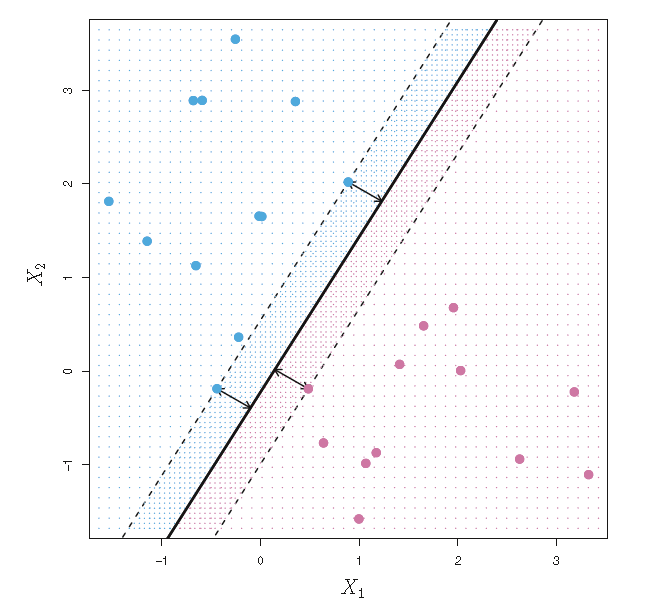
\includegraphics[width=0.45\textwidth]{imgs/svm_hiperplanos.png}
\caption{ Ejemplo de hiperplano calculado por SVM. Los puntos que están a menor distancia del hiperplano separador se denominan vectores soporte. Créditos: Drew Wilimitis, \url{towardsdatascience.com} }
\label{fig:svm-hiperplanos}
\end{figure}
    
    \item La contra es que puede no existir un hiperplano que los separe, por ejemplo, si las clases se encuentran ``demasiado superpuestas'' en el especio de atributos. Ver figura \ref{fig:svm-imposible}.
    
\begin{figure}[h!]
\centering
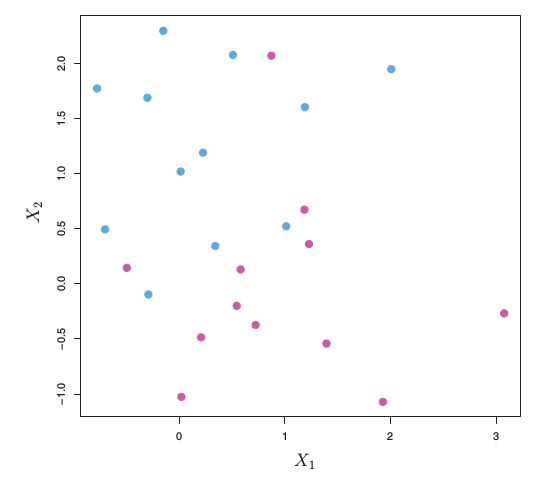
\includegraphics[width=0.45\textwidth]{imgs/svm_imposible.png}
\caption{ En este ejemplo de clases celestes y violetas, no pueden ser separadas por un hiperplano. Créditos: Drew Wilimitis, \url{towardsdatascience.com} }
\label{fig:svm-imposible}
\end{figure}
    
    \item Podemos debilitar el problema de separar las clases utilizando márgenes ``relajados'' y permitiendo a algunos puntos de entrenamiento estar dentro del lado equivocado del hiperplano. Ver figura \ref{fig:svm-margenes}.

\begin{figure}[h!]
\centering
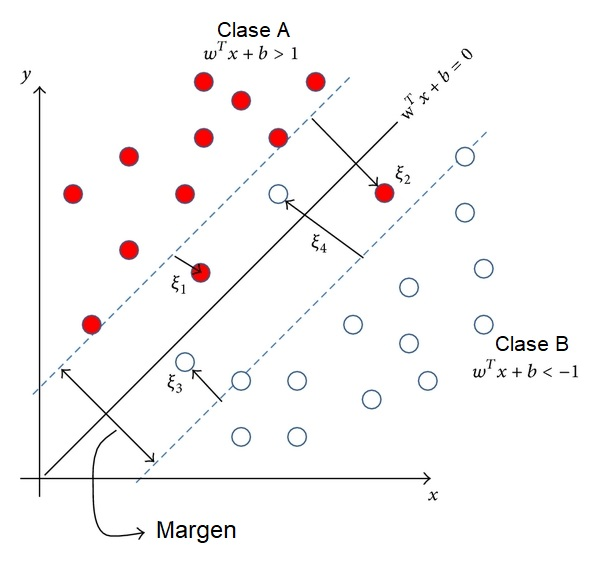
\includegraphics[width=0.6\textwidth]{imgs/svm_margenes.png}
\caption{ Los valores notados como $\epsilon_i$ constituyen una medida de margen relajado para cada ejemplo y se denominan \textit{variables slack}.
El hiperparámetro C permite regular cuán permisivo es el modelo a la hora de permitir errores de clasificación. Imagen tomada de \cite{svm-margenes}. }
\label{fig:svm-margenes}
\end{figure}    

    En la formulación matemática minimizaremos no sólo la distancia mínima al hiperplano separador sino también un término que pondere \textit{``que tanto nos permitimos relajar los márgenes''}. De aquí sale el hiperparámetro $C$ llamado \textit{coste} o \textit{regularización}.
    
    \item Seguimos teniendo el limitante de que las fronteras son sólo lineales: puede no ser lo ideal para muchas distribuciones de datos. Es por eso que se introduce una función $\phi$ que mapee los datos de la variable independiente $x$ a un espacio de mayor dimensionalidad donde potencialmente las clases serán separables por una frontera lineal. Así, trataremos de usar la formulación de hiperplano ya desarrollada hasta el punto anterior no para los datos $\{(x_i, y_i)\}$ sino para separar $\{(\phi(x_i), y_i)\}$. Ver figura \ref{fig:svm-kernel}.
    
\begin{figure}[h!]
\centering
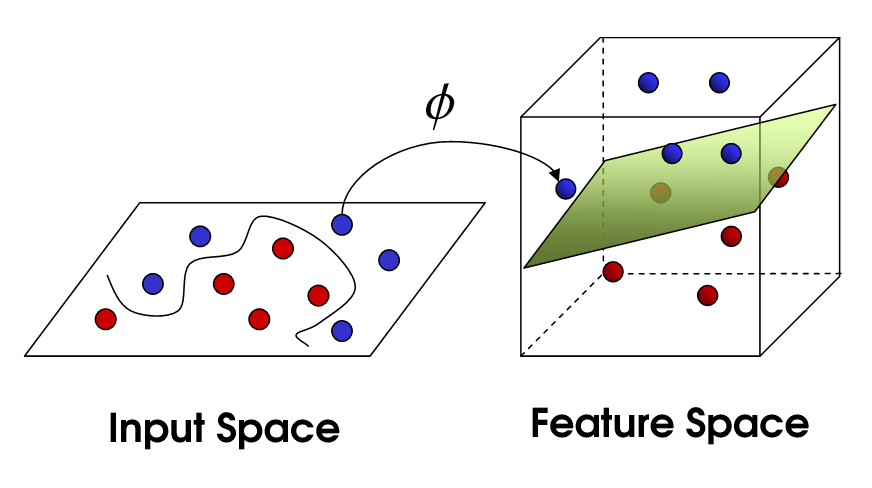
\includegraphics[width=0.6\textwidth]{imgs/svm_kernel.png}
\caption{ Luego de mapear los puntos por medio de una función no lineal a un espacio de mayor dimensionalidad pueden ser separados por un hiperplano. Remitiéndonos al espacio de atributos original el hiperplano constituye una superficie curva que particiona el espacio. Créditos: Drew Wilimitis, \url{towardsdatascience.com}  }
\label{fig:svm-kernel}
\end{figure}    
    
    \item El punto anterior no tiene sentido sin lo que se denomina \textbf{truco de kernel}: trabajando algebraicamente la fórmula a optimizar se llega a una expresión tal que nunca es necesario para la optimización calcular explícitamente el mapeo $\phi(x)$ sobre los ejemplos, sólo es necesario saber como calcular productos internos sobre el resultado de dichos mapeos (en el espacio de mayor dimensionalidad).
    
    O sea simplemente necesitamos saber como calcular:
    \begin{equation*}
        K(x_i, x_j) = <\phi(x_i), \phi(x_j)>
    \end{equation*}
    Donde $<,>$ es la operación de producto interno. Dicha función $K$ se denomina \textbf{función kernel}. Se desarrollan varias de estas funciones en la bilbiografía citada  que poseen un sustento teórico relevante. Su elección y la de sus parámetros constituyen hiperparámetros de las SVM.

\end{enumerate}

